\myChapter{Dependability e Security}\cite{tax}
I veicoli a guida autonoma appartengono alla categoria dei sistemi critici. Un sistema critico è un sistema il cui malfunzionamento può provocare danni
considerati inacettabili. Questi includono danni a oggetti di valore, danni ambientali e nei casi piu gravi, il ferimento o addirittura la morte delle persone.
Per garantire che un tale sistema operi nel modo più sicuro possibile è necessario analizzare tutti i fattori che possono portare a  un fallimento irreversibile.

La textbf{dependability} è la capacità di un sistema di fornire un servizio sul quale è possibile fare affidamento in modo giustificato.
Essa viene suddivisa in 3 categorie:
\begin{itemize}
    \item Attributi
    \item Minacce
    \item Mezzi di Raggiungimento
\end{itemize}
\begin{figure}[h]
    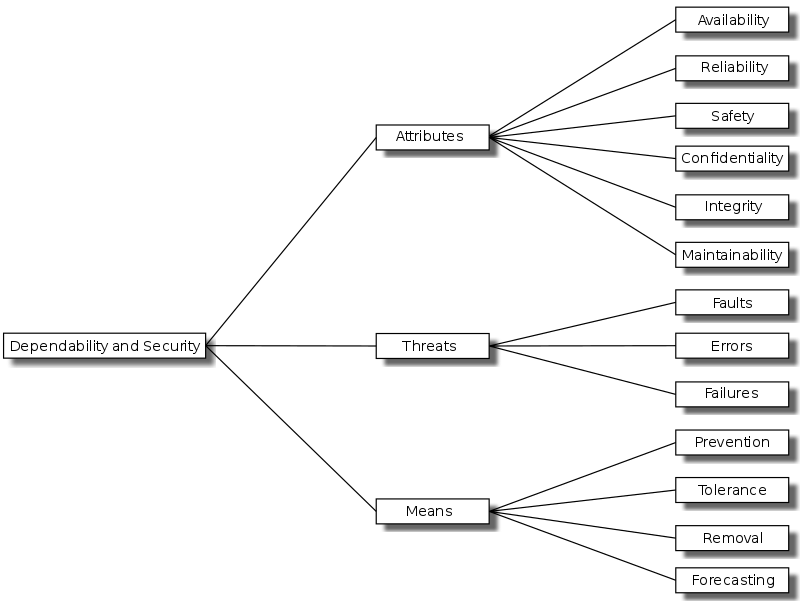
\includegraphics[width = \linewidth]{dep.png}
    \caption{tassonomia  della dependability\cite{dep}}
    \label{fig:dep}
\end{figure}
\section{Attributi}
La dependability comprende i seguenti attributi:
\begin{itemize}
    \item \textbf{availability}: disponibilità del servizio corretto
    \item \textbf{reliability}: stabilità del servizio corretto
    \item \textbf{safety}: assenza di conseguenze catastrofiche sullìutente e sull'ambiente
    \item \textbf{integrity}: assenza di alterazioni improprie al sistema
    \item \textbf{maintainability}: capacità di subire modifiche e riparazioni
\end{itemize}
Quando si considera la \textbf{security} è necessario specificare un ulteriore attributo: la confidentiality, ovvero la mancata divulgazione di informazioni non 
autorizzata. La security è composta da confidentiality, integrity e availability.
\section{Mezzi di raggiungimento}
Nel corso degli anni si sono sviluppate molte metodologie per raggiungere dependability e security. Tali metodologie possono essere raggruppate in quattro macrocategorie:
\begin{itemize}
    \item \textbf{fault prevention}: mezzi per prevenire l'occorrenza e l'introduzione di guasti
    \item \textbf{fault tolerance}: mezzi per evitare fallimenti di servizio quando sono presenti dei guasti
    \item \textbf{fault removal}: mezzi per ridurre numero e gravità dei guasti
    \item \textbf{fault forecasting}: mezzi per stimare numero, incidenza futura e probabili conseguenze di guasti
\end{itemize}
Fault prevention e fault tolerance portano al conseguimento della dependability mentre fault removal e fault forecasting sono i mezzi di validazione
\section{Minacce}
Le maggiori minacce per la dependability sono i \textbf{guasti}(faults in inglese). I guasti hanno varie cause e causano gli \textbf{errori}. Un errore può causarne altri fino a propagarsi
al di fuori dei confini del sistema. Quando ciò avviene, si verifica un \textbf{fallimento}. Un fallimento è la situazione in cui il servizio fornito
è diverso dal servizio corretto.
\begin{figure}[h]
    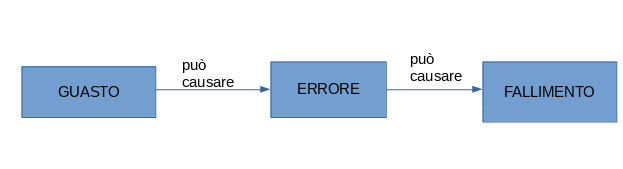
\includegraphics[width=\linewidth]{chain.png}
    \caption{Catena guasto-errore-fallimento}
\end{figure}
\subsection{Tipi di guasti}
I guasti vengono classificati secondo 8 parametri, i quali creano le classi di guasto elementari, mostrate in figura \ref{fig:tax}
\begin{figure}[h]
    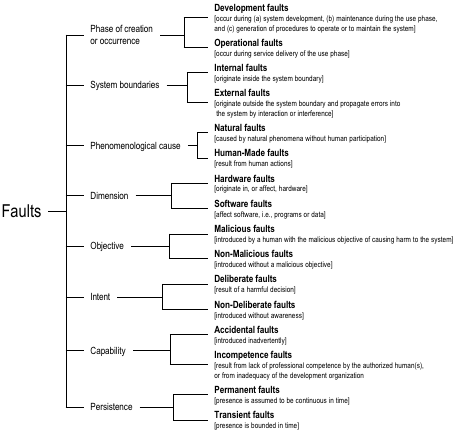
\includegraphics[width = \linewidth]{faults.png}
    \caption{tassonomia dei guasti\cite{tax}}
    \label{fig:tax}
\end{figure}
 I diversi tipi di guasto sono raggrupati in tre categorie:
 \begin{itemize}
     \item \textbf{Development faults}: i guasti che avvengono in fase di sviluppo
     \item \textbf{Physical faults}: i guasti che riguardano l'hardware
     \item \textbf{Interaction faults}: tutti i guasti causati dall'interazione con l'ambiente esterno
 \end{itemize}
 \newpage
 \subsubsection{Guasti causati dall'azione umana}
 I guasti sul quale ci concentriamo sono quelli di origine umana volontari. Questi guasti possono essere causati da una mancanza di 
 azioni ove necessarie(omission faults), oppure da azioni che si rilevano essere sbagliate(commision faults). Questi guasti possono
 essere distinti in due tipi, sulla base dell'\emph{obbiettivo} dello sviluppatore o dell'essere umano che lo causa:
 \begin{itemize}
     \item guasti involontari, causati  accidentalmente senza lo scopo di arrecare danno
     \item guasti maligni, causati in modo volontario per arrecare danni al sistema durante l'uso
 \end{itemize}
 I guasti maligni hanno  come scopo la negazione del servizio(denial of service), l'accesso a informazioni confidenziali
 o la modifica impropria di un sistema.
 Vengono raggruppati in due classi:
 \begin{itemize}
     \item \textbf{guasti a livello logico}: comprendono virus, worms, bombe logiche ecc.
     \item \textbf{tentativi di intrusione}, anche usando mezzi fisici
 \end{itemize}
 In entrambi i casi si sfrutta una vulnerabilità di un sistema per ottenerne il pieno controllo(exploit).
 La vulnerabilità solitamente è a livello software ed è causata dall'azione involontaria degli sviluppatori.

